\documentclass[tikz,border=2pt]{standalone}
\usepackage{tikz}
\usetikzlibrary{positioning}
\begin{document}
% Namikawa--Ueno type: I_{l-0-0}
% Target MRNC type: I_{l,g1}
% Adapted from Tim Dokchitser picture: I_{{\it n},g1}
% Parameter substitution: n -> l
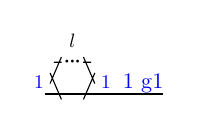
\begin{tikzpicture}[xscale=0.57,yscale=0.62]
\draw[thick,shorten >=2] (-0.09,0)--(2.67,0) node[inner sep=2pt,blue,above left,scale=0.8] {1 \smash{g}1};
\draw[scale=0.8] (0,0) ++(0.05,0.3) node[anchor=east,blue,scale=0.7] {1} ++(0.3,-0.45)--++(115:0.75)++(295:0.15)++(245:0.15)--++(65:0.75)++(245:0.15)++(180:0.15)--++(0:0.22) ++(0:0.15) node{$\cdot$} ++(0:0.15) node{$\cdot$} node[above=0.1,anchor=south,scale=0.7]{$l$}++(0:0.15) node{$\cdot$} ++(0:0.15) --++(0:0.22)++(180:0.15)++(115:0.15)--++(295:0.75)++(115:0.15)++(65:0.15)--++(245:0.75)++(0.3,0.45) node[anchor=west,blue,scale=0.7] {1};\end{tikzpicture}
\end{document}
